\documentclass[10pt,journal]{IEEEtran}

\usepackage{amsmath,amssymb,amsfonts}
\usepackage{array}
\usepackage{booktabs}
\usepackage{multirow}
\usepackage{tabularx}
\usepackage{cite}
\usepackage{url}
\usepackage{graphicx}
\usepackage{xspace}
\usepackage{xcolor}
\usepackage{tikz}
\usetikzlibrary{arrows.meta,positioning,shapes.geometric,fit,calc}
\usepackage[caption=false,font=footnotesize]{subfig}
\usepackage[ruled,vlined,linesnumbered]{algorithm2e}
\usepackage[hypertexnames=false]{hyperref}

\hypersetup{colorlinks=true,linkcolor=blue,citecolor=blue,urlcolor=blue}

\newtheorem{proposition}{Proposition}

\newcommand{\method}{NARCIS\xspace}
\newcommand{\bits}{\mathrm{bpc}}
\newcolumntype{Y}{>{\raggedright\arraybackslash}X}

\begin{document}

\title{NARCIS: Authenticated Neural Coverless Image Signaling
  with Attack-Qualified Codebooks and Error Correction}

\author{\emph{St\'{e}phane Ga\"{e}l R.}~Ekodeck,
        \emph{Vivien Beyala}~Kamgang,
        \emph{Serge Alain}~Eb\'{e}l\'{e},
        and~\emph{Julius Marcellin}~Nkenlifack,~\IEEEmembership{Member,~IEEE}
\thanks{This research received no external funding. The authors declare no
  competing interests. WYSAWIS, cited in the related work, shares authors
  with this study and is explicitly identified as such; it is used as
  published qualitative context, not as an experimental baseline.
  \emph{(Corresponding author: St\'ephane Ga\"el R.~Ekodeck,
  stephane-gael.ekodeck@facsciences-uy1.cm.)}}
\thanks{S.~G.~R.~Ekodeck is with the Department of Computer Science,
  LIRIMA, TEAM GRIMCAPE, University of Yaound\'e~I, Yaound\'e, Cameroon;
  IRD, UMI~209 UMMISCO, IRD France Nord, 93143 Bondy, France; and
  Sorbonne Universit\'e, UMI~209 UMMISCO, 75005 Paris, France.
  (ORCID: 0000-0002-8094-8832)}
\thanks{V.~B.~Kamgang and J.~M.~Nkenlifack are with RTU Mathematics and
  Computer Science, The University of Bertoua, Bertoua, Cameroon, and
  RUFCEA (UR-IFIA), University of Dschang, Dschang, Cameroon.
  (ORCID: 0000-0002-3644-1866; 0000-0003-3322-4687)}
\thanks{S.~A.~Eb\'el\'e is with the Department of Computer Science,
  LIRIMA, TEAM GRIMCAPE, University of Yaound\'e~I, Yaound\'e, Cameroon;
  IRD, UMI~209 UMMISCO, IRD France Nord, 93143 Bondy, France; and
  Sorbonne Universit\'e, UMI~209 UMMISCO, 75005 Paris, France.
  (ORCID: 0000-0001-7036-7068)}}

\markboth{IEEE Transactions on Multimedia}%
{Ekodeck \MakeLowercase{\textit{et al.}}: NARCIS: Authenticated
  Neural Coverless Image Signaling}

\maketitle

% ---------------------------------------------------------------
\begin{abstract}
Selection-based coverless steganography communicates by transmitting
unchanged natural images chosen from a shared index. Two gaps limit its
operational viability: existing systems neither verify that a finite
qualified index can satisfy a specific message \emph{before}
transmission, nor provide a fully authenticated, replay-resistant,
error-correcting protocol. This paper presents \method~(Neural Adaptive
Robust Coverless Image Signaling) and makes three contributions.
\emph{(i)~Feasible operating point criterion}: a codebook is accepted
only when every attack-qualified bucket satisfies the multiplicity
required by every protected coded message; the selected alphabet is the
largest consistent with this criterion.
\emph{(ii)~End-to-end coverless pipeline}: a self-supervised encoder
trained with a variance--invariance--covariance objective maps images to
normalised 64-dimensional descriptors; a quantile codebook provides
balanced symbol classes; multi-attack qualification (12 calibration
transforms) removes geometrically unstable covers; a calibration-locked
projection search raises the minimum stable bucket from 92 to~161 while
maintaining full recovery; AES-GCM authenticates payloads and session
metadata; a keyed Gray permutation limits symbol exposure; Reed--Solomon
coding corrects residual label errors.
\emph{(iii)~Systematic detectability and ablation evaluation}: three
detector classes are applied over five partitions each of BOSSBase-1.01
and Caltech-101; on BOSSBase all confidence intervals include chance;
on Caltech-101 a weak reproducible shift is confirmed (20-repeat CNN
mean~AUC~0.533, 95\%~CI~[0.517, 0.548]); removing qualification
reduces complete-message success from 210/210 to 142/210~(67.6\%).
Across 1{,}575 trials under clean, calibration, and holdout conditions,
\method recovered every authenticated plaintext (mean symbol accuracy
98.74\% on BOSSBase, 98.59\% on Caltech-101). Net throughput at
$K{=}16$ scales from 0.184 to 1.213~bits per cover for 8- to
128-byte payloads.
\end{abstract}

\begin{IEEEkeywords}
Coverless image steganography, neural image descriptor, robust
codebook, authenticated encryption, error correction, cover
selection, Reed-Solomon, AES-GCM.
\end{IEEEkeywords}

% ---------------------------------------------------------------
\section{Introduction}
\label{sec:introduction}

\IEEEPARstart{S}{election-based} coverless image steganography
communicates information by choosing natural images from a shared
index rather than by modifying a carrier. The transmitted objects are
unaltered photographs. Three interconnected gaps limit this approach's
operational viability.

\textbf{Gap~1: Finite-index message feasibility is not verified before
transmission.} Existing methods report nominal hash length or average
symbol accuracy. Neither metric guarantees that the required sequence
of symbols can be satisfied by the available, qualified index for a
given message. A transmission that cannot be realised fails silently
rather than signalling infeasibility, producing message-dependent
coverage gaps that are invisible in per-symbol statistics
\cite{zhou2015coverless,meng2024review}.

\textbf{Gap~2: No end-to-end coverless protocol integrates
authentication, replay control, and error correction.} Selection-based
schemes propose that cover integrity replaces steganographic hiding, but
they leave payload confidentiality, metadata authenticity, replay
rejection, and channel error recovery as open problems. The published
literature treats these components individually or omits them entirely
within the coverless framework \cite{zheng2017hashing,li2024surf,
guo2025diverse,guo2026capacity}.

\textbf{Gap~3: Cover stability filtering creates unquantified selection
bias.} Retaining only stable covers changes the distribution of
transmitted images relative to the full index. Whether this selection
leaks detectable information depends on the dataset, the filtering
policy, and the detector, but this three-way dependence is rarely
measured \cite{fridrich2012rich,cachin1998steganography}.

\method~(Neural Adaptive Robust Coverless Image Signaling) closes all
three gaps simultaneously.

\textbf{Contribution~1: Feasible operating point.} A codebook is
accepted only when every attack-qualified bucket satisfies the
multiplicity required by each protected coded message. The selected
operating point is the largest alphabet consistent with this criterion.
Across 1{,}575 end-to-end trials on two datasets and 21 channel
conditions, \method recovered 100\% of authenticated plaintexts.

\textbf{Contribution~2: End-to-end coverless pipeline.} A
self-supervised encoder trained with a variance--invariance--covariance
objective maps images to normalised 64-dimensional descriptors. A
quantile codebook partitions the principal descriptor direction into
balanced symbol classes. Multi-attack qualification (12 calibration
transforms) removes geometrically unstable covers; a calibration-locked
projection search increases the minimum stable bucket from 92 to~161
while maintaining 210/210 recoveries~(BOSSBase seed~11).
AES-GCM~\cite{nist2007gcm} authenticates payloads and session metadata
with associated sender-receiver identities; a keyed Gray permutation
limits symbol-to-label exposure; monotonic sequence checking rejects
replay; Reed-Solomon coding~\cite{reed1960polynomial} corrects residual
label errors. Net throughput at $K{=}16$ scales from 0.184 to
1.213~bits per cover for 8- to 128-byte
payloads~(Section~\ref{subsec:scalability}).

\textbf{Contribution~3: Systematic detectability and ablation
evaluation.} Three detector classes (global logistic regression,
residual-feature ExtraTrees, and a selection CNN) are applied to five
partitions of each dataset. On BOSSBase all confidence intervals include
chance performance. On Caltech-101 a weak reproducible shift is
confirmed (20-repeat CNN mean~AUC~0.533, 95\%~CI~[0.517, 0.548]),
reported transparently. A matched ablation on BOSSBase seed~11
establishes attack qualification as the dominant robustness mechanism:
removing it reduces complete-message success from 210/210 to
142/210~(67.6\%), with crop and large-rotation conditions failing
entirely~(Section~\ref{subsec:detect}).

The remainder of the paper is organised as follows. Section~\ref{sec:related}
reviews related work. Section~\ref{sec:model} states the system and threat
model with formal security propositions. Section~\ref{sec:method}
presents the \method components. Section~\ref{sec:experiments} describes
the experimental protocol. Section~\ref{sec:results} reports all results.
Section~\ref{sec:discussion} interprets them. Section~\ref{sec:conclusion}
concludes.

% ---------------------------------------------------------------
\section{Related Work}
\label{sec:related}

\subsection{Hash- and retrieval-based coverless communication}

Early coverless systems mapped robust image hashes to message fragments
\cite{zhou2015coverless,zheng2017hashing}. Later retrieval-based schemes
used local descriptors to improve resistance to common processing
\cite{li2024surf}. These methods preserve the transmitted image, but
the database must contain sufficiently many stable representatives for
every message symbol.

Abdulsattar~\cite{abdulsattar2021} increased single-image nominal
capacity by dividing a grayscale cover into overlapping blocks and
mapping eigenvalue comparisons to ASCII values. WYSAWIS~\cite{wysawis2025}
groups 15-bit block hashes into 16 sequence categories and uses
cloud-file rankings to represent segments. Both works illustrate that
a large nominal representation space does not by itself guarantee
per-message feasibility under finite-index constraints.

\subsection{Learned, joint, and stability-aware methods}

Neural feature mapping and generation provide semantic representations
or larger message spaces \cite{qin2020gan,meng2024review}. Selection
and generation have been combined with StarGAN \cite{chen2022stargan},
while information-driven generation has been applied to control
message-to-content mappings \cite{zhang2023idgan}. Recent semantic
approaches derive symbols from neglected objects, human poses, or
detections \cite{zou2023neglected,tan2024pose,meng2024object}. Other
systems use semantic text-to-image generation or latent diffusion to
enlarge the generative cover space \cite{li2025semantic,guo2026diffusion}.

Ren and Wu~\cite{ren2024joint} combined selection and generation modules
to address mapping completeness and reconstruction. Guo
et~al.~\cite{guo2025diverse} studied robustness and diversity against
passive and active analysis. Guo and Ping~\cite{guo2026capacity} used
pseudo-Zernike moments, stability-aware quantisation, and
stability-regularised clustering, reporting average robustness of
99.54\%, 98.64\%, and 97.19\% at 10, 14, and 15 bits on Holidays,
VOC, and ImageNet, respectively. These results use different datasets,
attack sets, and protocol overheads; direct numerical comparison
with \method is not attempted, and the cited figures serve as
qualitative context.

\method shares the stability-aware objective but focuses on protocol
completeness rather than descriptor-level capacity: its primary
evaluation unit is complete authenticated message recovery under a
finite qualified index.

\subsection{Security and evaluation}

No pixel modification removes embedding artefacts, but it does not
establish communication security. Selection may alter the distribution
of transmitted content, and metadata can reveal protocol state.
Steganalysis research has shown that weak statistical differences can
be exploitable \cite{fridrich2012rich,holub2014uniward,
xu2016steganalysis,ye2017steganalysis,yedroudj2018net,
boroumand2018srnet}. Formal steganographic security distinguishes
distributional secrecy from cryptographic payload protection
\cite{cachin1998steganography}. \method therefore separates
cryptographic mechanisms (Propositions~\ref{prop:conf} and
\ref{prop:auth}) from empirical selection detectability
(Section~\ref{subsec:detect}).

Table~\ref{tab:taxonomy} separates existing families by cover
formation, mapping mechanism, and protocol-level protection.

\begin{table*}[t]
\centering
\caption{Structural comparison of coverless image-steganography
  families. ``Protocol protection'' denotes integrated authenticated
  payload handling and error correction rather than image-level
  robustness alone.}
\label{tab:taxonomy}
\small
\begin{tabularx}{\textwidth}{p{2.5cm}p{2.4cm}p{3.0cm}p{3.0cm}Y}
\toprule
Family & Representative works & Cover formation &
Mapping / descriptor & Protocol protection\\
\midrule
Block/hash mapping &
Abdulsattar~\cite{abdulsattar2021}; WYSAWIS~\cite{wysawis2025} &
Existing natural images &
Block comparisons or category hashes &
Not central to the cited mapping mechanism\\
Retrieval and local features &
Li et~al.~\cite{li2024surf} &
Selected natural images &
SURF-based retrieval &
Not central to the cited retrieval mechanism\\
Adversarial generation &
Qin et~al.~\cite{qin2020gan}; Chen et~al.~\cite{chen2022stargan};
Zhang et~al.~\cite{zhang2023idgan} &
Generated or selected/generated images &
Latent or information-driven neural mapping &
Evaluated mainly at image/message mapping level\\
Semantic mapping &
Zou et~al.~\cite{zou2023neglected}; Tan et~al.~\cite{tan2024pose};
Meng et~al.~\cite{meng2024object} &
Existing natural images &
Objects, poses, or detector outputs &
Not the primary contribution\\
Text-to-image and diffusion &
Li et~al.~\cite{li2025semantic}; Guo et~al.~\cite{guo2026diffusion} &
Generated images &
Semantic prompts or latent transformations &
Not directly comparable to finite-index retrieval\\
Stability-aware selection &
Guo et~al.~\cite{guo2025diverse}; Guo-Ping~\cite{guo2026capacity} &
Selected natural images &
Stable handcrafted features and clustering &
Image-level robustness and diversity\\
\method & This work &
Selected unchanged natural images &
Invariant neural descriptor and qualified quantile codebook &
AES-GCM, replay control, Reed-Solomon, exact recovery\\
\bottomrule
\end{tabularx}
\end{table*}

% ---------------------------------------------------------------
\section{System and Threat Model}
\label{sec:model}

\subsection{Shared index and protocol parties}

The sender and receiver share an indexed corpus
$\mathcal{I}=\{(x_i,y_i)\}_{i=1}^{N}$, a symbol-assignment key $k_s$,
a payload encryption key $k_p$, and a metadata seal key $k_m$. Each
$x_i$ is a natural image and $y_i\in\{0,\ldots,K-1\}$ is its codebook
label. The sender transmits a sequence of unchanged images; the receiver
applies the same descriptor and codebook to recover labels and decode
the protected payload.

\subsection{Channel model}

The channel may apply JPEG compression, additive Gaussian noise,
Gaussian blur, resizing, central cropping, or small rotations. The
declared channel model determines which calibration transformations are
used to qualify covers and train the descriptor.

\subsection{Protocol targets}

The protocol enforces five properties:
(i)~\emph{cover integrity}: no pixel modification by the sender;
(ii)~\emph{message correctness}: exact plaintext recovery or explicit
     failure;
(iii)~\emph{confidentiality and authenticity}: authenticated
     encryption of payload and metadata;
(iv)~\emph{freshness}: rejection of replayed or reordered sequences;
(v)~\emph{channel robustness}: correction of residual label errors
    within the Reed-Solomon budget.

\subsection{Formal security properties}

The following propositions state the cryptographic guarantees
provided by \method under standard assumptions. They follow directly
from the authenticated encryption security of AES-GCM~\cite{nist2007gcm}
and require no new cryptographic proof.

\begin{proposition}[Payload Confidentiality]
\label{prop:conf}
For plaintext $m$, nonce derived from sequence number $n$, and key $k_p$
unknown to the adversary, the ciphertext
$c=\operatorname{AEAD.Enc}_{k_p}(m;\,\mathrm{nonce},\mathrm{AD})$
is computationally indistinguishable from a uniformly random string of
the same length, with advantage bounded by the IND-CCA2 security of
AES-GCM~\cite{nist2007gcm}. An adversary observing transmitted images
and sealed metadata gains no information about $m$.
\end{proposition}

\begin{proposition}[Authenticity and Replay Rejection]
\label{prop:auth}
A message is accepted by the receiver only when
(i)~the AES-GCM tag on the sealed metadata verifies under $k_m$
    with sender-receiver identities as associated data, and
(ii)~the sequence number $n$ embedded in the metadata satisfies
    $n>n_{\max}$, where $n_{\max}$ is the highest previously accepted
    value for that sender. Under AES-GCM's authentication
    guarantee~\cite{nist2007gcm}, any altered or replayed message
    fails condition~(i) or condition~(ii).
\end{proposition}

Traffic analysis and semantic inference from image content remain
outside the cryptographic claim. Selection detectability is treated
as a measured empirical property~(Section~\ref{subsec:detect}).

% ---------------------------------------------------------------
\section{NARCIS Method}
\label{sec:method}

\subsection{Channel-invariant neural descriptor}

Channel transformations are applied at the declared channel resolution,
and the resulting images are resized to $128\times128$ for descriptor
inference. The encoder has four convolutional blocks with 16, 32, 64,
and 96 channels; each block uses two $3\times3$ convolutions, batch
normalisation, and SiLU activations; the last three blocks downsample
by a factor of two. Global average pooling and a two-layer
$96\to128\to64$ projection head produce a 64-dimensional unit-normalised
descriptor $z=f_\theta(x)$. The grayscale and RGB instances have 231{,}312
and 231{,}600 trainable parameters, respectively; only the first
convolution differs. Fig.~\ref{fig:encoder} shows the implemented
dimensions.

Training uses two independently distorted views $x^{(1)}$ and $x^{(2)}$
of the same image. Each view is generated by randomly selecting JPEG
compression, Gaussian noise, blur, resize, crop, rotation, or the
identity transform. The loss is
\begin{equation}
\mathcal{L}=
\lambda_{\mathrm{inv}}\mathcal{L}_{\mathrm{inv}}+
\lambda_{\mathrm{var}}\mathcal{L}_{\mathrm{var}}+
\lambda_{\mathrm{cov}}\mathcal{L}_{\mathrm{cov}},
\label{eq:loss}
\end{equation}
where $\mathcal{L}_{\mathrm{inv}}$ is the mean squared distance between
paired descriptors, $\mathcal{L}_{\mathrm{var}}$ prevents dimensional
collapse, and $\mathcal{L}_{\mathrm{cov}}$ penalises off-diagonal
covariance. This variance-invariance-covariance structure follows the
non-contrastive principle of VICReg \cite{bardes2022vicreg}. The weights
are $(\lambda_{\mathrm{inv}},\lambda_{\mathrm{var}},\lambda_{\mathrm{cov}})
=(25,25,1)$; the target standard deviation is $64^{-1/2}$, consistent
with unit-normalised descriptors.

For a batch of $B$ paired $d$-dimensional descriptors $Z$ and $Z'$:
\begin{align}
\mathcal{L}_{\mathrm{inv}}&=\frac{1}{Bd}\lVert Z-Z'\rVert_F^2,\\
\mathcal{L}_{\mathrm{var}}&=\frac{1}{d}\sum_{j=1}^{d}
\bigl[\max(0,\gamma-\sigma_j(Z))+
\max(0,\gamma-\sigma_j(Z'))\bigr],\\
\mathcal{L}_{\mathrm{cov}}&=\frac{1}{d(d-1)}\sum_{i\ne j}
\bigl(C_{ij}(Z)^2+C_{ij}(Z')^2\bigr),
\end{align}
where $\gamma=d^{-1/2}$, $\sigma_j$ is the batch standard deviation
with $10^{-4}$ variance regularisation, and
$C(Z)=(Z-\bar Z)^\top(Z-\bar Z)/(B-1)$.

\begin{figure*}[t]
\centering
\resizebox{\textwidth}{!}{%
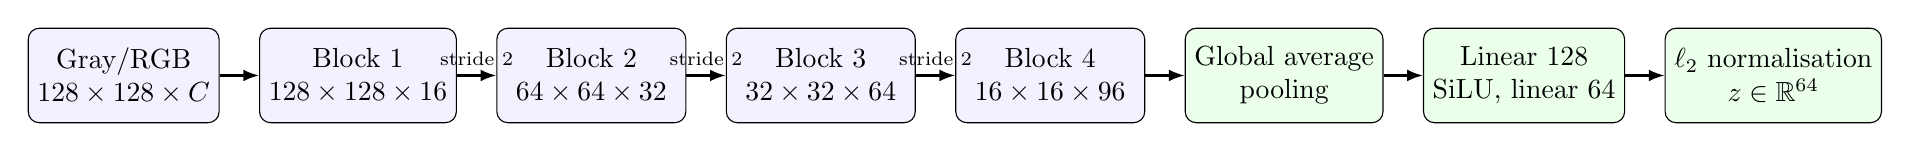
\begin{tikzpicture}[
  node distance=5mm,
  layer/.style={draw, rounded corners, align=center, minimum height=12mm,
    minimum width=24mm, fill=blue!5},
  head/.style={draw, rounded corners, align=center, minimum height=12mm,
    minimum width=21mm, fill=green!8},
  arrow/.style={-{Latex[length=2mm]}, thick}
]
\node[layer] (input) {Gray/RGB\\$128\times128\times C$};
\node[layer, right=of input] (b1) {Block 1\\$128\times128\times16$};
\node[layer, right=of b1] (b2) {Block 2\\$64\times64\times32$};
\node[layer, right=of b2] (b3) {Block 3\\$32\times32\times64$};
\node[layer, right=of b3] (b4) {Block 4\\$16\times16\times96$};
\node[head, right=of b4] (gap) {Global average\\pooling};
\node[head, right=of gap] (proj) {Linear 128\\SiLU, linear 64};
\node[head, right=of proj] (norm) {$\ell_2$ normalisation\\$z\in\mathbb{R}^{64}$};
\draw[arrow] (input)--(b1);
\draw[arrow] (b1)--node[above, font=\scriptsize]{stride 2}(b2);
\draw[arrow] (b2)--node[above, font=\scriptsize]{stride 2}(b3);
\draw[arrow] (b3)--node[above, font=\scriptsize]{stride 2}(b4);
\draw[arrow] (b4)--(gap);
\draw[arrow] (gap)--(proj);
\draw[arrow] (proj)--(norm);
\end{tikzpicture}%
}
\caption{Descriptor encoder used in both principal evaluations, with $C{=}1$
for BOSSBase and $C{=}3$ for Caltech-101. Each convolutional block contains
two $3\times3$ convolution-batch-normalisation-SiLU stages; channels
transformations precede model resizing to $128\times128$.}
\label{fig:encoder}
\end{figure*}

\subsection{Balanced quantile codebook}

Let $Z\in\mathbb{R}^{N\times64}$ contain clean descriptors and let
$v_1$ be the first right singular vector of the centred matrix. Each
descriptor is projected as
\begin{equation}
s_i=(z_i-\bar z)^\top v_1.
\end{equation}
For a candidate alphabet of size $K$, boundaries are placed at the
empirical quantiles $j/K$, $j=1,\ldots,K-1$. The resulting label is
\begin{equation}
q_K(z_i)=\sum_{j=1}^{K-1}\mathbf{1}[s_i>b_j].
\label{eq:quantile}
\end{equation}
Quantile partitioning balances clean occupancy before channel
qualification and avoids empty clusters from unconstrained fitting.
In the reduced sensitivity experiment, PC1 explained 72.90\% of
descriptor variance; Section~\ref{subsec:sensitivity} analyses
alternative projections.

\subsection{Attack-qualified cover index}

A cover is retained only when its label is unchanged under every
calibration condition:
\begin{equation}
\mathcal{S}_K=
\bigl\{i:q_K(f_\theta(T(x_i)))=q_K(f_\theta(x_i)),
\ \forall T\in\mathcal{T}_{\mathrm{cal}}\bigr\}.
\label{eq:stable}
\end{equation}
The calibration set $\mathcal{T}_{\mathrm{cal}}$ contains 12
transformations: JPEG qualities 80 and 50; Gaussian noise standard
deviations 5 and 12; blur radii 0.8 and 1.5; resize factors 0.75
and 0.50; crop fractions 0.05 and 0.10; rotations of $3^\circ$
and $7^\circ$.

Seven image statistics are used to estimate selection bias: mean,
standard deviation, horizontal and vertical gradient magnitude,
entropy, and the 0.1 and 0.9 intensity quantiles. Within each symbol
bucket, stable covers are ordered by clipped inverse-propensity
weighted random priorities. This does not change labels or pixels; it
reduces deterministic preference for visually distinctive stable covers.

\subsection{Protected message representation}

For plaintext $m$ and sequence number $n$, AES-GCM produces
\begin{equation}
c=\operatorname{AEAD.Enc}_{k_p}(m;\,\mathrm{nonce},
\texttt{NARCIS-PAYLOAD-1}\Vert n).
\end{equation}
The ciphertext envelope is framed with a protocol marker, length field,
and CRC-32, then encoded with Reed-Solomon parity
\cite{reed1960polynomial}. Session metadata contains the sequence
number, padding, codebook size, and cover count; it is independently
sealed with AES-GCM using sender and receiver identities as associated
data. The receiver accepts only a sequence number greater than the
highest previously accepted value for that sender~(Proposition~\ref{prop:auth}).

For $K=2^b$, the coded bit stream is divided into $b$-bit symbols. A
keyed permutation combines a Gray ordering, a key-derived cyclic shift,
and a key-derived orientation. Let
$h=\operatorname{HMAC\text{-}SHA256}(k_s,\texttt{cluster-order})$~\cite{nist2008hmac},
$a=\operatorname{int}(h_{0:8})\bmod K$, and $r{=}{-1}$ if the least
significant bit of $h_8$ is one, otherwise $r{=}1$. For position
$p\in\{0,\ldots,K-1\}$, define the binary-reflected Gray symbol
$g(p)=p\oplus(p\!\gg\!1)$ and
\begin{equation}
\pi_k(g(p))=(a+rp)\bmod K.
\label{eq:keyedgray}
\end{equation}
Adjacent symbol values remain adjacent in the unshifted codebook order,
while the externally observed symbol-to-label assignment depends on the
key.

\subsection{Feasible operating point}

Let $d_k(c)$ denote the number of occurrences of label $k$ required
to transmit envelope $c$, and let $a_k$ be the number of unused
qualified covers in bucket $k$. A candidate codebook is feasible when
\begin{equation}
d_k(c)\leq a_k,\qquad
\forall k,\ \forall c\in\mathcal{C}_{\mathrm{eval}}.
\label{eq:feasibility}
\end{equation}
Candidate sizes are evaluated from largest to smallest. The selected
operating point is the largest $K$ satisfying~\eqref{eq:feasibility}.
This criterion distinguishes nominal symbol capacity $\log_2 K$ from
the net payload rate after encryption, framing, and error correction.

\subsection{Computational complexity}

Let $N$ be the index size, $A{=}|\mathcal{T}_{\mathrm{cal}}|$, $d$
the descriptor dimension, $K$ the alphabet size, $L$ the cover count,
and $F_\theta$ the encoder inference cost. Clean embedding costs
$O(NF_\theta)$. Multi-attack qualification is the dominant offline
term, $O(ANF_\theta{+}AN\log K)$ with binary search over sorted
boundaries. PCA fitting costs $O(Nd^2)$; sorting projected values
$O(N\log N)$. Online cover retrieval and keyed mapping are $O(L)$
with pre-built buckets; Reed-Solomon decoding adds a fixed block cost.
Offline qualification is intentionally amortised across subsequent
transmissions.

Fig.~\ref{fig:pipeline} separates the offline index-construction phase
from online protected transmission and recovery. Algorithm~\ref{alg:narcis}
summarises the transmission and recovery steps.

\begin{figure*}[t]
\centering
\resizebox{\textwidth}{!}{%
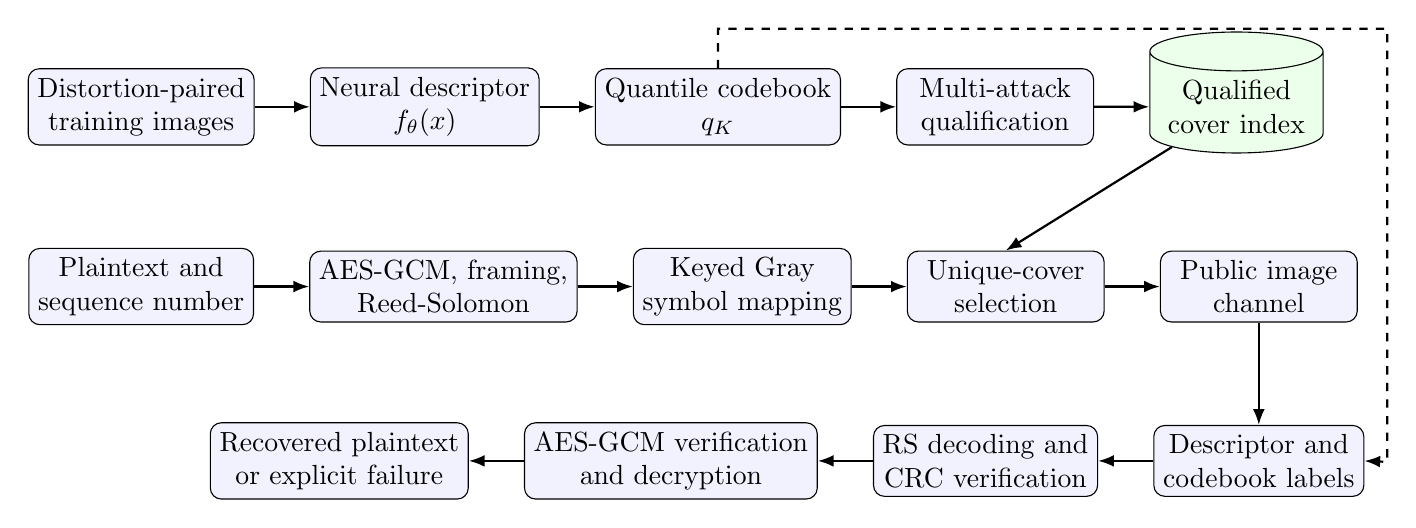
\begin{tikzpicture}[
  node distance=5mm and 7mm,
  box/.style={draw, rounded corners, align=center, minimum height=9mm,
    minimum width=25mm, fill=blue!5},
  store/.style={draw, cylinder, shape border rotate=90, aspect=0.25,
    align=center, minimum height=11mm, minimum width=22mm, fill=green!8},
  arrow/.style={-{Latex[length=2mm]}, thick},
  dashedarrow/.style={-{Latex[length=2mm]}, thick, dashed}
]
\node[box] (train)   {Distortion-paired\\training images};
\node[box, right=of train]   (encoder)  {Neural descriptor\\$f_\theta(x)$};
\node[box, right=of encoder] (quantile) {Quantile codebook\\$q_K$};
\node[box, right=of quantile](qualify)  {Multi-attack\\qualification};
\node[store, right=of qualify](index)   {Qualified\\cover index};

\node[box, below=13mm of train]   (payload) {Plaintext and\\sequence number};
\node[box, right=of payload]  (aead)    {AES-GCM, framing,\\Reed-Solomon};
\node[box, right=of aead]     (mapping) {Keyed Gray\\symbol mapping};
\node[box, right=of mapping]  (select)  {Unique-cover\\selection};
\node[box, right=of select]   (channel) {Public image\\channel};

\node[box, below=13mm of channel] (classify) {Descriptor and\\codebook labels};
\node[box, left=of classify]  (decode)  {RS decoding and\\CRC verification};
\node[box, left=of decode]    (decrypt) {AES-GCM verification\\and decryption};
\node[box, left=of decrypt]   (output)  {Recovered plaintext\\or explicit failure};

\draw[arrow] (train)--(encoder);
\draw[arrow] (encoder)--(quantile);
\draw[arrow] (quantile)--(qualify);
\draw[arrow] (qualify)--(index);
\draw[arrow] (payload)--(aead);
\draw[arrow] (aead)--(mapping);
\draw[arrow] (mapping)--(select);
\draw[arrow] (index)--(select.north);
\draw[arrow] (select)--(channel);
\draw[arrow] (channel)--(classify);
\draw[arrow] (classify)--(decode);
\draw[arrow] (decode)--(decrypt);
\draw[arrow] (decrypt)--(output);
\draw[dashedarrow] (quantile.north)--++(0,0.5cm)--++(8.5cm,0)
  --++(0,-5.5cm)--(classify.east);
\end{tikzpicture}%
}
\caption{\method construction and transmission pipeline. Index
construction and qualification are performed offline. The transmitted
objects are unchanged images selected from the qualified index.}
\label{fig:pipeline}
\end{figure*}

\begin{algorithm}[t]
\caption{\method protected coverless transmission}
\label{alg:narcis}
\KwIn{Plaintext $m$, sequence $n$, qualified index $\mathcal{I}$, keys}
\KwOut{Recovered plaintext or failure}
Encrypt $m$ with sequence-bound AES-GCM\;
Frame the ciphertext and apply Reed-Solomon coding\;
Select the largest feasible codebook $K$\;
Map coded symbols to labels with the keyed permutation $\pi_k$\;
Select one unused qualified cover for each required label\;
Transmit the unchanged cover sequence and sealed metadata\;
Verify metadata and reject replayed sequence numbers\;
Classify received covers and invert the keyed mapping\;
Apply Reed-Solomon decoding and verify CRC\;
Authenticate and decrypt the payload\;
\Return plaintext if every verification succeeds; otherwise failure\;
\end{algorithm}

% ---------------------------------------------------------------
\section{Experimental Protocol}
\label{sec:experiments}

\subsection{Datasets and partitions}
\label{subsec:datasets}

The principal evaluation uses BOSSBase~1.01~\cite{bas2011boss},
containing 10{,}000 grayscale photographs at $512\times512$ pixels.
For each seed in $\{11,29,47,71,101\}$, a deterministic permutation
provides 2{,}000 training images and a disjoint 8{,}000-image cover
index.

Cross-dataset validation uses Caltech-101~\cite{fei2004caltech}:
9{,}144 natural RGB images from 101 object categories with variable
source resolutions, centre-fitted to $256\times256$ for batching. Each
of the same five seeds assigns 1{,}500 images to descriptor training
and 7{,}000 disjoint images to the shared index. Semantic labels are
used neither in training nor in codebook construction.

CIFAR-100~\cite{krizhevsky2009cifar} is retained only for the
controlled descriptor-comparison ablation~(Section~\ref{subsec:ablation}):
three seeds, 2{,}000 training images, an 8{,}000-image index, three
messages per seed.

The encoder is trained separately on each partition for five epochs
with AdamW, batch size~16, learning rate~$10^{-3}$, and weight
decay~$10^{-5}$. BOSSBase evaluates ten eight-byte plaintexts per
seed; Caltech-101 evaluates five. Reed-Solomon coding uses 128 parity
bytes. Symbol repetition is set to one; redundancy is instead provided
by byte-level parity, which avoids multiplying the required 348-464
cover sequences. The two principal campaigns comprise 75 protected
messages and 1{,}575 message-condition trials.

\subsection{Channel conditions and metrics}

The 12 calibration transformations are those in~\eqref{eq:stable}.
Eight holdout strengths are evaluated only at test time: Gaussian
noise standard deviations 9 and 15; blur radii 1.2 and 1.8; crop
fractions 0.08 and 0.12; and rotations of $5^\circ$ and $9^\circ$.
Together with the clean channel, this yields 21 conditions.

Two metrics are reported: (i)~\emph{symbol accuracy}, the fraction of
transmitted covers assigned to their intended labels after channel
processing; (ii)~\emph{complete-message success}, which is~1 only when
error correction, CRC verification, authenticated decryption, and
plaintext equality all succeed.

Confidence intervals are two-sided 95\% Student-$t$ intervals over the
five seed-level values. They quantify variation across deterministic
partitions and do not imply coverage over datasets or untested channels.

\subsection{Baselines, descriptor comparison, and ablation}
\label{subsec:ablation}

\textit{Local descriptor baselines.} A normalised $16\times16$
low-frequency DCT descriptor and a normalised 64-bin grayscale
histogram are subjected to the same quantile partition, calibration
attacks, candidate codebook sizes, and protected-message feasibility
rule as \method. Neither descriptor receives invariance training.
Under these conditions, neither the DCT nor the histogram formed a
feasible codebook at \emph{any} candidate alphabet size ($K\in
\{64,32,16,8,4,2\}$) in any of the three CIFAR-100 partitions. This
outcome demonstrates that VICReg-style invariance training is a
necessary prerequisite for the multi-attack qualification stage to
produce a non-empty feasible codebook, not merely a preference that
improves capacity.

\textit{Qualification ablation.} The main ablation removes attack-based
cover qualification while retaining the same neural descriptor, codebook
size, protected messages, and decoder. It is applied to two settings:
(a)~the three-seed CIFAR-100 protocol, where it is computationally
efficient to measure across all conditions, and (b)~BOSSBase seed~11
with a matched 10-message, 21-condition protocol to confirm the
BOSSBase result directly~(Section~\ref{subsec:ablation_results}).

\textit{Repetition factor check.} A second check confirms the
configured repetition factor of one.

\subsection{Selection detectability}
\label{subsec:detect_proto}

A logistic regression on seven global image statistics (mean, standard
deviation, two gradient magnitudes, entropy, and two intensity quantiles)
distinguishes selected from non-selected index images using a stratified
65/35 train/test split. A second detector extracts 52 high-pass residual
co-occurrence summaries inspired by rich-model steganalysis
\cite{fridrich2012rich} and applies an ExtraTrees ensemble. A third
detector is a lightweight selection CNN trained for eight epochs on
$64\times64$ views. The AUC measures detectability for all three. To
assess the stability of the CNN estimate on the most sensitive partition
(Caltech-101 seed~47), 20 independent training runs are performed.

\subsection{Sensitivity and projection analysis}
\label{subsec:sens_proto}

A targeted reduced experiment (seed~11, 500 training images, 1{,}500-image
index, three epochs, $96\times96$ inputs) compares descriptor dimensions
32, 64, and 128; three loss-weight configurations; and projections on
the first three principal directions plus a fixed random direction.

A separate seed-11 full-protocol analysis evaluates 16 PCA directions
(PC1-PC16) and 32 independent random projections to characterise the
relationship between descriptor variance and stability under
calibration attacks.

% ---------------------------------------------------------------
\section{Results}
\label{sec:results}

\subsection{Codebook feasibility}

Table~\ref{tab:config_boss} reports the selected BOSSBase configurations.
Four partitions supported 16 symbols (4~bits per cover); seed~47
supported eight symbols (3~bits per cover). Between 30.38\% and 48.73\%
of the index remained stable under all 12 calibration attacks.
Table~\ref{tab:config_cal} reports the Caltech-101 configurations; all
five partitions selected $K{=}16$.

Each eight-byte plaintext required 348 covers at 4~bits per cover and
464 at 3~bits per cover. The measured net plaintext rates were 0.184
and 0.138 bits per transmitted cover, including encryption, framing,
and error correction.

\begin{table}[t]
\centering
\caption{Selected BOSSBase operating points on 8{,}000-image indices.}
\label{tab:config_boss}
\footnotesize
\resizebox{\columnwidth}{!}{%
\begin{tabular}{rrrrrr}
\toprule
Seed & $K$ & bpc & Stable & Min.\ bucket & Median bucket\\
\midrule
11  & 16 & 4 & 2{,}823 (35.3\%) & 92  & 164\\
29  & 16 & 4 & 2{,}430 (30.4\%) & 61  & 154\\
47  & 8  & 3 & 3{,}898 (48.7\%) & 177 & 510\\
71  & 16 & 4 & 2{,}687 (33.6\%) & 80  & 155\\
101 & 16 & 4 & 2{,}846 (35.6\%) & 99  & 146\\
\bottomrule
\end{tabular}%
}
\end{table}

\begin{table}[t]
\centering
\caption{Selected Caltech-101 operating points on 7{,}000-image RGB
  indices. All five partitions selected $K{=}16$.}
\label{tab:config_cal}
\footnotesize
\resizebox{\columnwidth}{!}{%
\begin{tabular}{rrrrr}
\toprule
Seed & Stable & Min.\ bucket & Median bucket & Max.\ bucket\\
\midrule
11  & 1{,}678 (24.0\%) & 38 & 104 & 203\\
29  & 1{,}540 (22.0\%) & 31 & 82  & 185\\
47  & 2{,}432 (34.7\%) & 76 & 160 & 218\\
71  & 2{,}289 (32.7\%) & 45 & 110 & 284\\
101 & 1{,}895 (27.1\%) & 35 & 89  & 214\\
\bottomrule
\end{tabular}%
}
\end{table}

\subsection{End-to-end robustness}

All 1{,}050 BOSSBase trials succeeded across five seeds, ten messages,
and 21 conditions. Mean symbol accuracy was 98.74\%. The two most
difficult holdout conditions were crop~12\% (84.37\%) and rotation
$9^\circ$ (91.75\%); the worst individual accuracy was 81.61\%.
Reed-Solomon corrected at most 61 byte positions per message block,
and authenticated decryption recovered every plaintext. The clean
channel, both JPEG settings, both resize settings, calibrated crops,
both blur calibration settings, and rotations up to $3^\circ$ produced
100\% mean symbol accuracy.

Fig.~\ref{fig:attacks} shows per-condition means for BOSSBase. All
525 Caltech-101 message-condition trials also recovered the
authenticated plaintext. Mean symbol accuracy was 98.59\%; the worst
individual accuracy was 79.89\% under the unseen 12\% crop;
Reed-Solomon corrected at most 63 byte positions. Fig.~\ref{fig:crossrobust}
compares the two datasets condition by condition.

\begin{figure}[t]
\centering
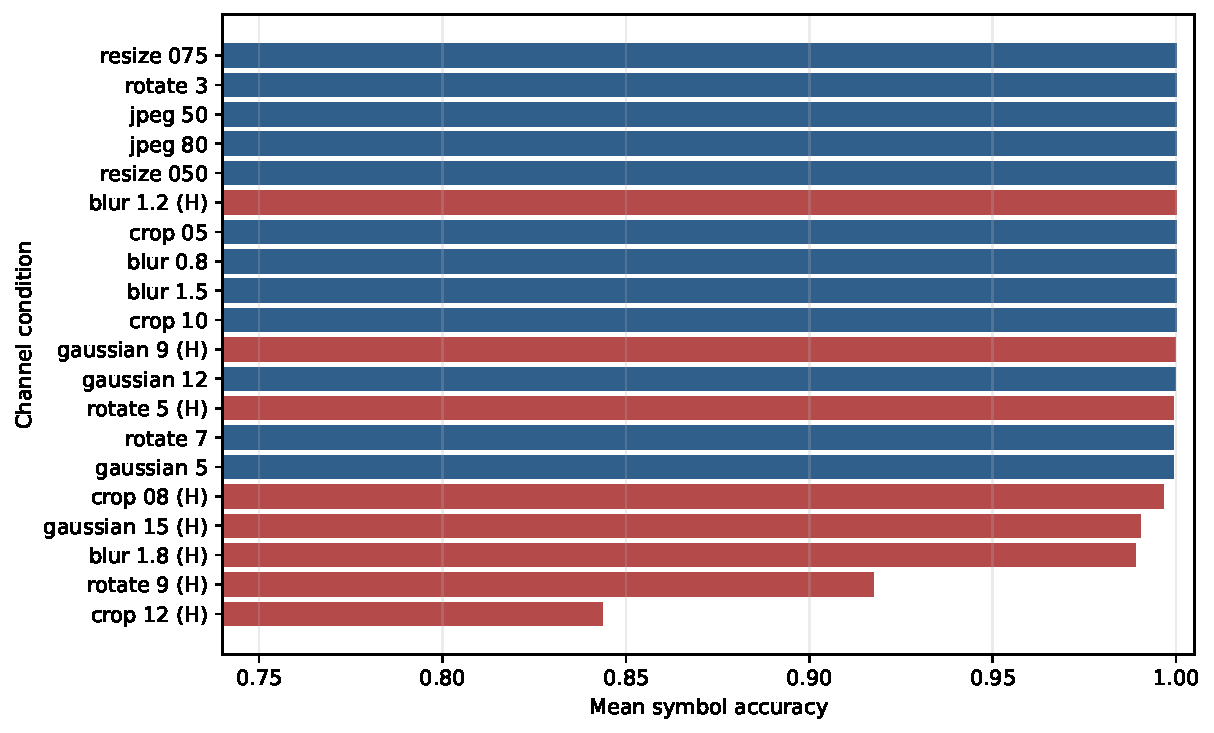
\includegraphics[width=\linewidth]{figures/Fig_04.pdf}
\caption{Mean BOSSBase symbol accuracy over five seeds and ten messages
  per seed. Holdout strengths were excluded from codebook qualification.
  Complete-message success was 100\% for every condition.}
\label{fig:attacks}
\end{figure}

\begin{figure*}[t]
\centering
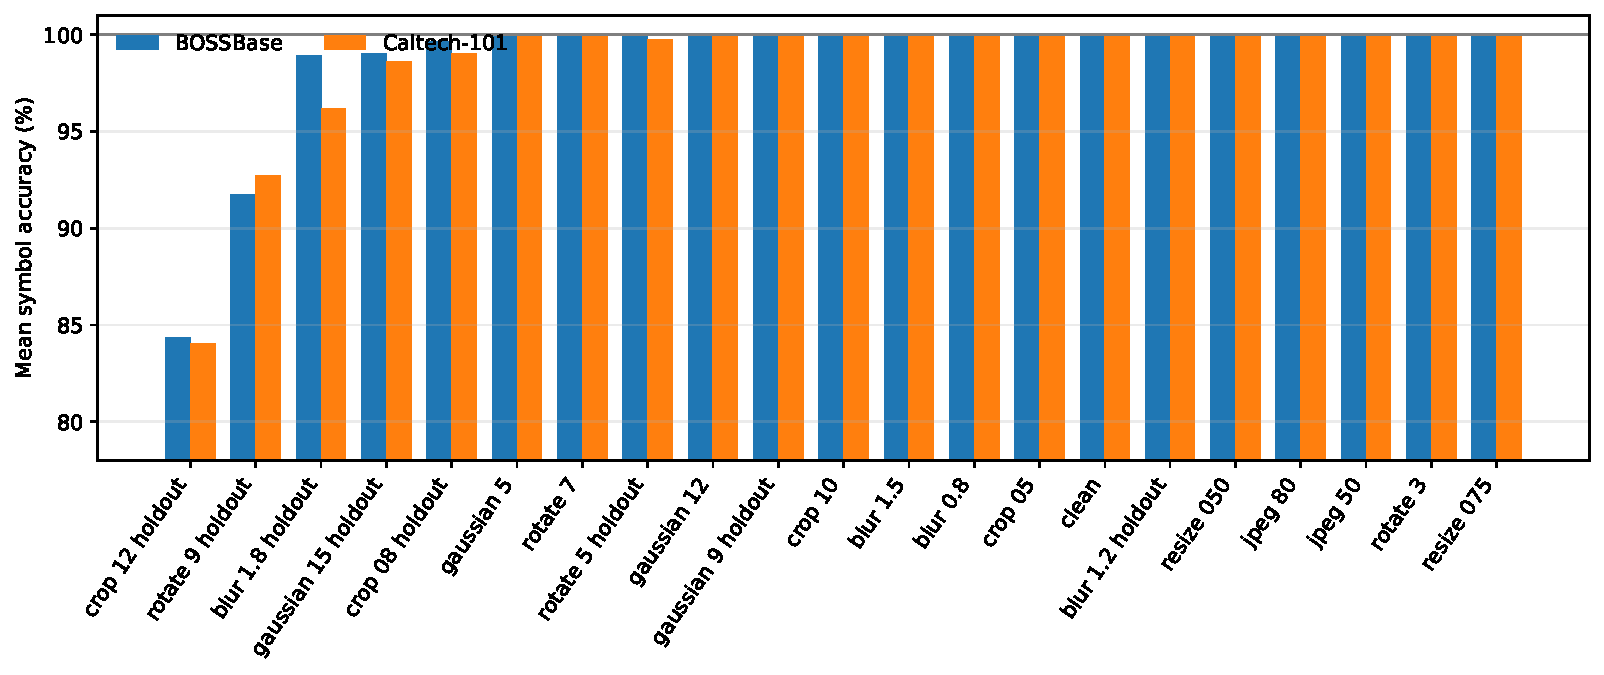
\includegraphics[width=\textwidth]{figures/Fig_05.pdf}
\caption{Mean symbol accuracy across five BOSSBase and five Caltech-101
  partitions. Calibration and holdout conditions use the same declared
  strengths. All 1{,}575 complete-message trials succeeded.}
\label{fig:crossrobust}
\end{figure*}

\subsection{Payload scalability}
\label{subsec:scalability}

Table~\ref{tab:scalability} reports the implemented overhead breakdown
and net throughput at $K{=}16$ for 8-, 32-, and 128-byte plaintexts.
AES-GCM adds a 12-byte nonce and 16-byte authentication tag; protocol
framing adds 10 bytes. For 8- and 32-byte payloads, a single
Reed-Solomon block with 128 parity bytes suffices; 128-byte payloads
span two blocks, doubling the effective parity to 256 bytes. Net
throughput therefore scales sub-linearly with overhead: from 0.184
bits per cover at 8 bytes to 0.646 at 32 bytes and 1.213 at 128 bytes.
Fig.~\ref{fig:scalability} illustrates this scaling. The short-payload
regime evaluating 8-byte messages in the principal campaigns represents
an extreme overhead case; longer practical payloads achieve meaningfully
higher efficiency under identical cryptographic and coding settings.

\begin{table}[t]
\centering
\caption{Payload scalability at $K{=}16$ (4 bits per cover).
  AES-GCM overhead: 12-byte nonce + 16-byte tag. Framing: 10~bytes.
  Two RS blocks are required for 128-byte payloads.}
\label{tab:scalability}
\footnotesize
\resizebox{\columnwidth}{!}{%
\begin{tabular}{rrrrrr}
\toprule
Payload & AES-GCM & RS blocks & Coded & Covers & Net bpc\\
(bytes) & (bytes) & ($\times$128 parity) & (bytes) & required &\\
\midrule
8   & 36  & 1 & 174 & 348 & 0.184\\
32  & 60  & 1 & 198 & 396 & 0.646\\
128 & 156 & 2 & 422 & 844 & 1.213\\
\bottomrule
\end{tabular}%
}
\end{table}

\begin{figure}[t]
\centering
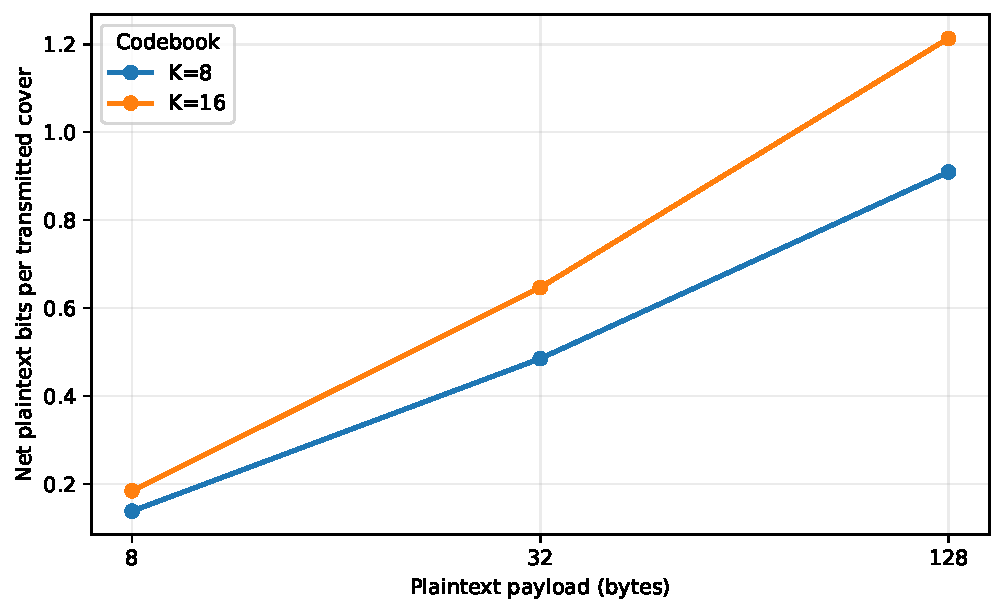
\includegraphics[width=\linewidth]{figures/Fig_03.pdf}
\caption{Net plaintext throughput (bits per cover) as a function of
  payload size at $K{=}16$. Overhead (AES-GCM, framing, RS parity)
  is amortised across larger payloads; the 128-byte point uses two
  RS blocks with 128 parity bytes each.}
\label{fig:scalability}
\end{figure}

\subsection{Training convergence}

Fig.~\ref{fig:convergence} reports the five-epoch training histories
for BOSSBase. The final loss values ranged from 0.066 (seed~47) to
0.157 (seed~29), a 2.4$\times$ spread that reflects variation in
partition character rather than training instability. Individual curves
are not monotonic because each epoch samples new distortion pairs.

\begin{figure}[t]
\centering
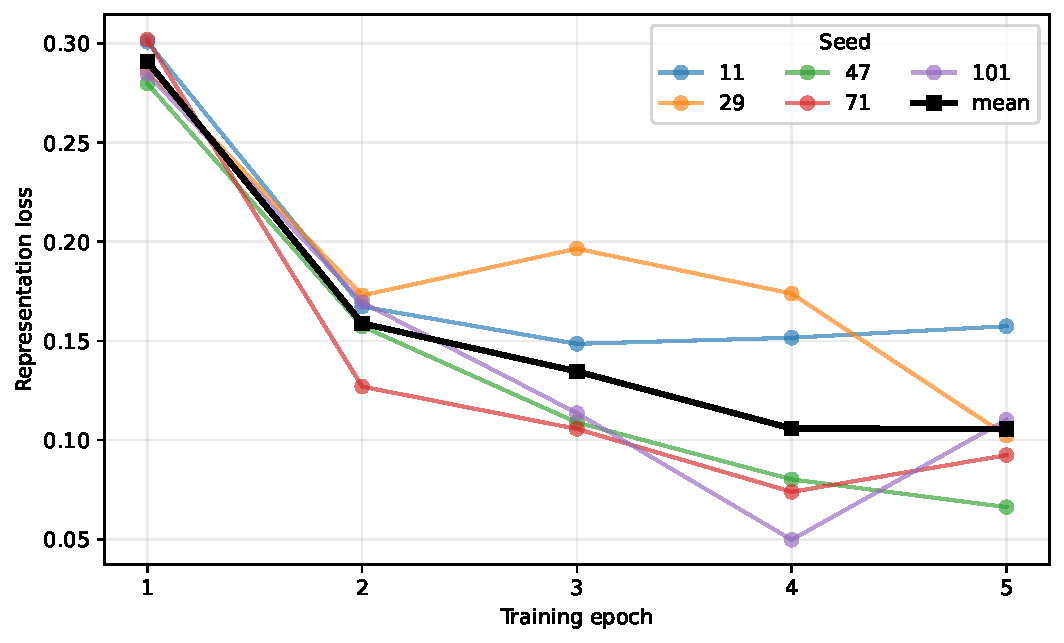
\includegraphics[width=\linewidth]{figures/Fig_06.pdf}
\caption{BOSSBase training loss for the five deterministic partitions.
  Non-monotonicity reflects fresh distortion-pair sampling each epoch.}
\label{fig:convergence}
\end{figure}

\subsection{Selection detectability}
\label{subsec:detect}

Table~\ref{tab:detect} reports the mean AUC and 95\% Student-$t$
confidence intervals over five partitions for each detector and dataset.

\begin{table}[t]
\centering
\caption{Selection-detection AUC (mean and 95\% Student-$t$ CI over
  five partitions). Intervals excluding 0.5 indicate a measurable shift.}
\label{tab:detect}
\footnotesize
\begin{tabular}{lll}
\toprule
Detector & BOSSBase & Caltech-101\\
\midrule
Global logistic     & 0.518 [0.489, 0.547] & 0.531 [0.504, 0.557]\\
Residual ExtraTrees & 0.514 [0.486, 0.543] & 0.533 [0.504, 0.562]\\
Selection CNN       & 0.515 [0.463, 0.566] & 0.530 [0.481, 0.579]\\
\bottomrule
\end{tabular}
\end{table}

On BOSSBase, all three confidence intervals include 0.5. On
Caltech-101, the two classical detectors show a small dataset-specific
selection shift (intervals exclude 0.5); the CNN five-partition
interval is wider and includes 0.5.

To assess whether the CNN result is stable on the most sensitive
partition, 20 independent training runs were performed on Caltech-101
seed~47. Fig.~\ref{fig:cnn_repeats} plots the resulting AUC
distribution. The 20-run mean is 0.533 (95\% CI [0.517, 0.548]),
which excludes 0.5. This confirms a small but reproducible
partition-specific selection signal on seed~47; Section~\ref{subsec:security}
places this finding in context.

\begin{figure}[t]
\centering
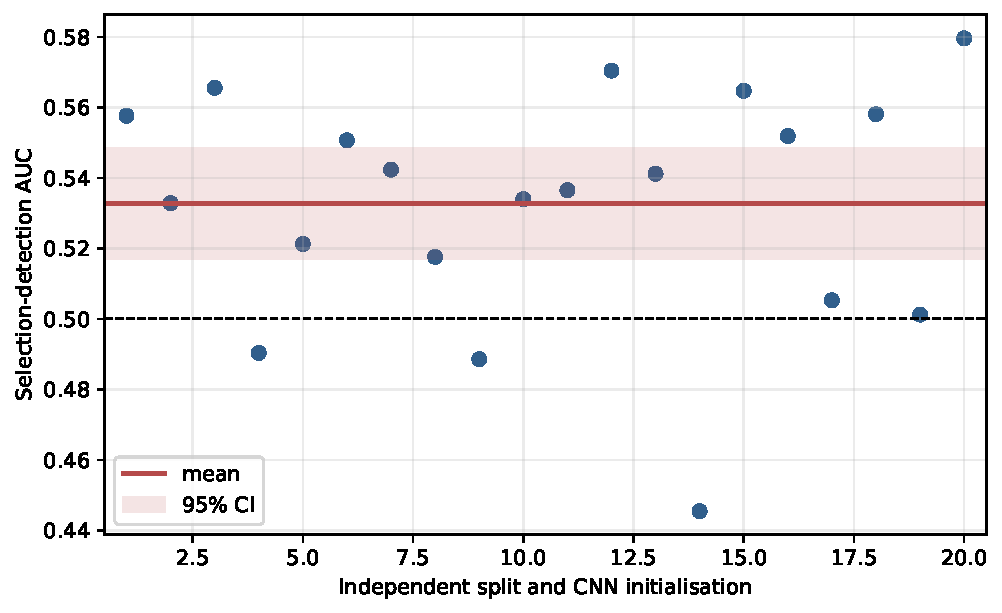
\includegraphics[width=\linewidth]{figures/Fig_08.pdf}
\caption{Distribution of selection-CNN AUC over 20 repeated
  independent training runs on Caltech-101 seed~47. The 20-run
  95\%~CI [0.517, 0.548] excludes chance performance; this is a
  partition-specific signal, not a protocol-level vulnerability.}
\label{fig:cnn_repeats}
\end{figure}

\subsection{Sensitivity, projection analysis, and complexity}
\label{subsec:sensitivity}

\textit{Configuration sensitivity.}
Table~\ref{tab:sensitivity} summarises the reduced sensitivity
experiment. Equal loss weights retained fewer stable covers and produced
the smallest minimum bucket. Dimension~128 improved retained stability
in this subset, but a confirmatory two-seed full-protocol run recovered
419/420 trials versus 420/420 for the corresponding 64-dimensional
runs. The 64-dimensional configuration is therefore retained.

\begin{table}[t]
\centering
\caption{Targeted sensitivity study on the reduced BOSSBase subset
  (seed~11, 1{,}500-image index, $96\times96$ inputs).}
\label{tab:sensitivity}
\small
\begin{tabular}{lrr}
\toprule
Configuration & Stable fraction & Min.\ bucket\\
\midrule
64D, 25/25/1  & 0.335 & 9\\
32D, 25/25/1  & 0.375 & 19\\
128D, 25/25/1 & 0.412 & 20\\
64D, 1/1/1    & 0.284 & 5\\
64D, 25/10/1  & 0.357 & 19\\
\bottomrule
\end{tabular}
\end{table}

\textit{Projection candidates.}
The sensitivity study used PC1 as the default projection direction.
Table~\ref{tab:projections} compares PC1 with PC2 and a survey of
random directions on the BOSSBase seed-11 full-protocol index
(8{,}000 images, $K{=}16$). PC1 and PC2 retain the same number of
stable images but PC2 produces a higher minimum bucket (115 vs.\ 92).
Among 32 randomly sampled fixed directions, the median minimum bucket
is 101 and the best observed is 161 (random\_15). A calibration-locked
search that selected the direction with the highest minimum bucket
before holdout evaluation achieved minimum bucket~161 and recovered
210/210 trials on seed~11. This single-partition result confirms the
direction analysis but does not replace the five-seed PC1 evaluation.
Fig.~\ref{fig:projections} plots minimum bucket against stable
fraction for all evaluated directions.

\begin{table}[t]
\centering
\caption{Projection candidates on BOSSBase seed-11 ($K{=}16$,
  8{,}000-image index). PC1 and PC2 retain the same stable images
  (2{,}823) but differ in bucket balance. The calibration-locked
  random direction (best of 32 trials) achieves the highest minimum
  bucket.}
\label{tab:projections}
\footnotesize
\resizebox{\columnwidth}{!}{%
\begin{tabular}{lllr}
\toprule
Direction & Expl.\ var. & Stable images & Min.\ bucket\\
\midrule
PC1                   & 94.07\% & 2{,}823 (35.3\%) &  92\\
PC2                   &  5.19\% & 2{,}823 (35.3\%) & 115\\
Random, median of 32  & ---     & 3{,}630 (45.4\%) & 101\\
Random, best of 32    & ---     & 3{,}867 (48.3\%) & 161\\
\bottomrule
\end{tabular}%
}
\end{table}

\begin{figure}[t]
\centering
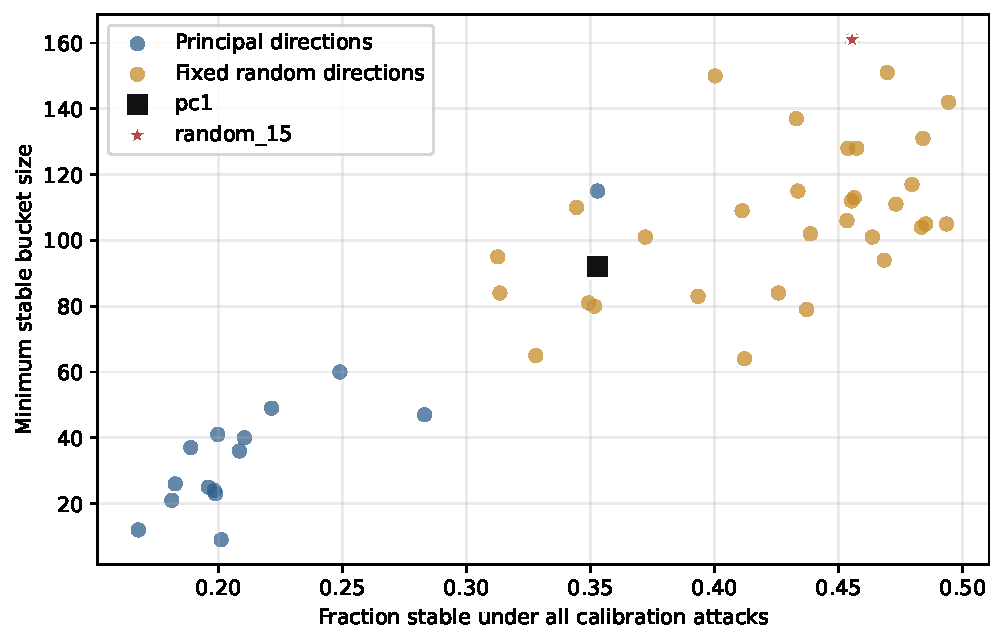
\includegraphics[width=\linewidth]{figures/Fig_09.pdf}
\caption{Minimum bucket size vs.\ stable fraction for PCA directions
  (PC1-PC16) and 32 random projections on BOSSBase seed-11.
  Random directions consistently dominate the PCA directions in
  minimum-bucket size, motivating attack-aware projection selection
  as a future extension.}
\label{fig:projections}
\end{figure}

\textit{Complexity.}
Native-image descriptor extraction averaged 87.83~s for 8{,}000 covers
(99.85~images/s). Calibration averaged 1{,}246.10~s per partition.
Complete evaluation averaged 754.63~s for 210 message-condition trials
(3.59~s per trial).

\subsection{Qualification ablation}
\label{subsec:ablation_results}

\textit{CIFAR-100 controlled ablation.}
The three-seed CIFAR-100 experiment recovered 189/189 protected
message-condition trials at $K{=}16$ (mean symbol accuracy~98.47\%).
Removing attack qualification reduced complete-message success
from 100\% to~43.65\%.

\textit{BOSSBase seed-11 matched ablation.}
Table~\ref{tab:ablation_boss} reports the per-condition results of the
matched BOSSBase seed-11 ablation (10~messages, 21~conditions). With
qualification (pc1-qualified), all 210/210 trials succeeded. Without
qualification (pc1-no-qualification), 142/210 trials succeeded
(67.6\%). Crop conditions failed completely (symbol accuracy 38-63\%,
far beyond the Reed-Solomon correction capacity of 64 bytes). Rotation
conditions at $\geq 7^\circ$ also failed outright. This confirms that
invariance training alone is insufficient: qualification is the
dominant robustness mechanism for distortions with sharp spatial
structure (crops, large rotations).

\begin{table*}[t]
\centering
\caption{BOSSBase seed-11 matched ablation: complete-message success over 10 messages
  per condition (21 conditions, 210 trials total). ``Qualif.''~=~pc1-qualified
  (\method standard); ``No qualif.''~=~pc1 without qualification. (H)~=~holdout strength.}
\label{tab:ablation_boss}
\small
\begin{tabular}{lccr}
\toprule
Condition & Qualif. & No qualif. & Mean sym.\ acc.\ (no qual.)\\
\midrule
Clean                      & 10/10 & 10/10              & 1.000 \\
JPEG 80, 50                & 10/10 & 10/10              & $>$0.993 \\
Gaussian $\sigma$5, 12     & 10/10 & 10/10              & 0.926-0.930 \\
Gaussian $\sigma$9~(H), 15~(H) & 10/10 & 10/10         & 0.925-0.926 \\
Blur 0.8, 1.5              & 10/10 & 10/10              & 0.872-0.950 \\
Blur 1.2~(H), 1.8~(H)     & 10/10 & 10/10              & 0.847-0.904 \\
Resize 0.75, 0.50          & 10/10 & 10/10              & 0.936-0.959 \\
Crop 5\%, 10\%             & 10/10 & \textbf{0/10}      & 0.430-0.627 \\
Crop 8\%~(H), 12\%~(H)    & 10/10 & \textbf{0/10}      & 0.381-0.524 \\
Rotate $3^\circ$           & 10/10 & 10/10              & 0.887 \\
Rotate $7^\circ$           & 10/10 & \textbf{0/10}      & 0.719 \\
Rotate $5^\circ$~(H)       & 10/10 & \textbf{2/10}      & 0.788 \\
Rotate $9^\circ$~(H)       & 10/10 & \textbf{0/10}      & 0.666 \\
\midrule
\textbf{Total}             & \textbf{210/210} & \textbf{142/210 (67.6\%)} & --- \\
\bottomrule
\end{tabular}
\end{table*}

\subsection{Position relative to published methods}

Table~\ref{tab:position} separates directly measured \method properties
from published context. Abdulsattar~\cite{abdulsattar2021} and
WYSAWIS~\cite{wysawis2025} provide high nominal intra-image or
category-based representations without end-to-end protocol evaluation.
Guo and Ping~\cite{guo2026capacity} report higher nominal capacities
and high average robustness on larger datasets, with a capacity
advantage at their operating points. \method's supporting position is
protocol completeness, not maximum nominal capacity.

\begin{table*}[t]
\centering
\caption{Positioning of \method. Values from different publications are
  not treated as a common-protocol ranking. (H) = holdout.}
\label{tab:position}
\small
\begin{tabularx}{\textwidth}{p{2.6cm}YYYY}
\toprule
Property &
Abdulsattar~\cite{abdulsattar2021} &
WYSAWIS~\cite{wysawis2025} &
Guo-Ping~\cite{guo2026capacity} & \method\\
\midrule
Representation & Eigenvalue comparisons in overlapping blocks &
15-bit block hashes, 16 category sequences &
PZM features, stability-aware quantisation and clustering &
Learned invariant descriptors with quantile codebook\\
Primary capacity & High nominal single-cover capacity &
High nominal block/category capacity &
10-15 bits on Holidays, VOC, ImageNet &
3-4 bits on BOSSBase; 4 bits on Caltech-101\\
Multi-attack qualification & Not evaluated & Not evaluated & Yes & Yes\\
Holdout attack strengths & Not evaluated & Not evaluated &
Not established from cited summary &
8 holdout strengths, 21 total conditions\\
Message-level error correction & Not reported & Not reported &
Not stated & Reed-Solomon; worst case 63 corrections\\
Authenticated payload + metadata & Not reported & Not reported &
Not stated & AES-GCM; replay guard; identity binding\\
Net throughput range & --- & --- & Not reported &
0.184-1.213 bpc (8-128 bytes at $K{=}16$)\\
Measured complete recovery & Not reported & Not reported &
Not directly comparable & 1{,}575/1{,}575 trials\\
\bottomrule
\end{tabularx}
\end{table*}

% ---------------------------------------------------------------
\section{Discussion}
\label{sec:discussion}

\subsection{What the experiments establish}

Four conclusions are supported. First, stable descriptor averages are
insufficient for communication: the multiplicity of every required
symbol must be verified. Second, cover qualification is the dominant
robustness component: removing it causes catastrophic failure on
cropping and large-rotation conditions that the neural descriptor alone
cannot tolerate. Third, forward error correction allows message
recovery at symbol accuracies well below 100\%. Fourth, cryptographic
verification changes the evaluation criterion: a trial succeeds only
when the exact plaintext is authenticated and recovered.

The five-seed results quantify finite-index and cross-corpus
variability. The same rules yield a feasible 16-symbol alphabet on
four BOSSBase partitions and an eight-symbol alphabet on one, while
all five Caltech-101 partitions support 16 symbols. Reporting the
lower BOSSBase operating point avoids selection of only favourable
partitions.

\subsection{Security interpretation}
\label{subsec:security}

Propositions~\ref{prop:conf} and~\ref{prop:auth} establish payload
confidentiality and metadata authenticity under AES-GCM. These
properties hold independently of whether selection is detectable.

The AUC experiments address a different question: whether the cover
selection policy creates a statistically detectable distribution
shift. The Caltech-101 classical detectors show mean AUCs of 0.531
and 0.533 with confidence intervals that exclude 0.5, indicating a
weak but real selection signal. The 20-repeat CNN result on the most
sensitive partition (mean 0.533, CI [0.517, 0.548]) confirms this
signal is reproducible.

These findings must be interpreted carefully. The shift is measured
against the full un-qualified index, not against an external cover
database. A warden who has access to the same index can therefore use
this signal. A warden who does not know the index must estimate the
reference distribution from publicly available images, which weakens
the detection advantage. The experiment establishes that the
qualification policy introduces a detectable selection leak on
Caltech-101 and motivates future work on distribution-preserving
selection strategies.

\subsection{Projection selection and the PC1 choice}
\label{subsec:projection}

Table~\ref{tab:projections} reveals a counter-intuitive finding:
PC1 (the direction of maximum descriptor variance) yields the lowest
minimum bucket~(92) among all evaluated projections on BOSSBase
seed~11. PC2 achieves the same stable-image count but a higher minimum
bucket~(115). The 32 random directions achieve substantially higher
stable fractions (median~45.4\%) and higher median minimum bucket
(101), with the best reaching~161.

This pattern arises because PC1 captures the descriptor dimensions
with the highest variance, and high-variance dimensions encode
precisely the visual content that is most perturbed by the channel
attacks. The calibration attacks therefore cause the largest
boundary-crossing rates along PC1. Lower-variance or random
directions encode less channel-sensitive content and retain more
stable covers as a result.

PC1 is retained in the principal evaluation because it is
deterministic, variance-maximising, and reproducible without
additional calibration data. A calibration-locked projection
(random\_15, minimum bucket~161) recovered 210/210 trials on seed~11,
confirming the gain is realisable. However, this single-partition
result does not replace the five-seed PC1 campaign, and an attack-aware
direction trained on calibration data while locked before holdout
evaluation is identified as the highest-priority future extension.

\subsection{Reed-Solomon parameter choice}
\label{subsec:rs}

The choice of 128 parity bytes per Reed-Solomon block is conservative
but verifiable. The maximum observed correction across all 1{,}575
trials was 63 byte positions~(Caltech-101), leaving a 1-byte margin
to the theoretical capacity of $\lfloor 128/2\rfloor{=}64$
correctable errors. The 128-byte payload evaluation uses two RS blocks,
each with 128 parity bytes, maintaining the same per-block correction
capacity while doubling the total parity overhead.

A tighter parameter (e.g., 64 parity bytes, $t{=}32$ corrections)
would halve the cover sequence length for short payloads but would
fail to correct the worst observed conditions~(BOSSBase seed~47 under
12\% crop: 61 corrections; Caltech-101 seed~29 crop~12\%: 63
corrections). The current choice is therefore the minimum that supports
the tested attack range with a measurable but non-zero margin.

\subsection{Comparative context}

Under the same quantile partition, attack set, candidate sizes, and
protected-message demand, neither the $16\times16$ DCT descriptor nor
the 64-bin histogram formed a feasible codebook at any tested alphabet
size. This is not a result about DCT and histogram methods in general;
it demonstrates that the VICReg invariance objective is a prerequisite
for the multi-attack qualification stage to produce a usable codebook
under the 12-attack calibration protocol. Without invariance training,
too few covers survive all calibration conditions to satisfy the
multiplicity constraint at any alphabet size.

Guo and Ping's stability-regularised clustering~\cite{guo2026capacity}
shares the objective of retaining stable covers but reports robustness
at the descriptor level on larger datasets with higher nominal
capacities. A direct comparison requires matching datasets, attack
definitions, and protocol overheads. The present results are
complementary rather than competitive: they characterise the
operating regime where the feasibility constraint is the binding
factor, whereas Guo-Ping target maximum nominal capacity at high
average robustness.

\subsection{Limitations}

The evaluation has four main limitations:
\begin{enumerate}
\item Caltech-101 adds variable-resolution RGB content, but its channel
input is centre-fitted to $256\times256$ for batching. Evaluation on
larger native-resolution colour corpora would test a broader regime.
\item The local baselines (DCT, histogram) isolate descriptor feasibility;
they are not faithful reimplementations of complete published coverless
systems.
\item The learned selection detector is a lightweight CNN designed for
the selected-vs.-non-selected task, not an SRNet reproduction.
Traffic-level sequence analysis is also outside this study.
\item PC1 is reproducible and variance-maximising but is not stability-optimal.
Attack-aware projection selection is identified as the highest-priority
future extension.
\end{enumerate}

% ---------------------------------------------------------------
\section{Conclusion}
\label{sec:conclusion}

\method integrates learned image descriptors, balanced codebooks,
attack-based cover qualification, keyed assignment, authenticated
encryption, replay control, and Reed-Solomon correction into one
selection-based coverless protocol. It recovered 1{,}050/1{,}050
protected message-condition trials on BOSSBase and 525/525 on RGB
Caltech-101, including eight holdout attack strengths. BOSSBase
supported 3-4 bits per cover; all Caltech-101 partitions supported
4~bits per cover. Mean symbol accuracies were 98.74\% and 98.59\%.

Net throughput at $K{=}16$ scales from 0.184 bits per cover for
8-byte payloads to 0.646 for 32-byte and 1.213 for 128-byte payloads,
demonstrating that the short-payload overhead is not a structural
limitation of the protocol. A matched BOSSBase seed-11 ablation
confirmed that removing qualification reduces complete-message success
from 210/210 to 142/210~(67.6\%), with crop and large-rotation
conditions failing completely. A calibration-locked projection recovered
210/210, motivating attack-aware direction selection as the
highest-priority extension.

Formal propositions ground the cryptographic protections in AES-GCM's
established security properties. Detectability is reported
transparently: BOSSBase shows no significant signal; Caltech-101 shows
a reproducible partition-specific CNN signal~(0.533, CI~[0.517,
0.548]) that identifies a selection leak attributable to the
qualification filter rather than to the protocol's cryptographic
components.

Three extensions follow from observed limits. First, attack-aware
projection selection should be trained on calibration data while locked
before holdout evaluation. Second, executable published-protocol
baselines should be evaluated under the same payload protection,
attacks, and finite-index demand. Third, larger native-resolution
colour corpora and traffic-level sequence detectors should extend the
present image-level analysis.

% ---------------------------------------------------------------
\section*{Acknowledgments}

This work was supported by the authors' institutions. No external
financial support was received.

% ---------------------------------------------------------------
\appendix

\section*{Data and Code Availability}

BOSSBase~1.01 is publicly available at \url{https://agents.fel.cvut.cz/boss/};
Caltech-101 at \url{https://data.caltech.edu/records/mzrjq-6wc02};
CIFAR-100 at \url{https://www.cs.toronto.edu/~kriz/cifar.html}.
The \method implementation, attack definitions, evaluation scripts,
fixed seeds, consolidated CSV and JSON result tables, and manuscript
sources are publicly available at
\url{https://github.com/EkodeckStephane/NARCIS}. Trained checkpoints
are not redistributed; the repository provides the commands to retrain.

% ---------------------------------------------------------------
\bibliographystyle{IEEEtran}
\bibliography{refs}

\end{document}
